% CpSc 855 - Final paper
% Takumi Bolte & Dan Welch - Spring 2014.
\documentclass{sig-alternate}

\usepackage{mathrsfs}
\usepackage{booktabs}
\usepackage{placeins}
\usepackage{graphicx}
\usepackage{subfigure}
\usepackage{listings}
\begin{document}
\conferenceinfo{Clemson 2014}{7th Clemson University Mini-Conference on Embedded Network Systems}
\title{An Extensible Approach to Verification of Embedded Network Systems*}

%Re-evaluating Verification of Embedded Network Systems:
%An Extensible Approach to Verification of Embedded Network Systems*}
\numberofauthors{2}
\author{
\alignauthor
%author
Daniel Welch\\
\affaddr{School of Computing, Clemson University}\\
\affaddr{Clemson, South Carolina, 29634}\\
\email{\texttt{\large{\{dtwelch\}@clemson.edu}}}
%author
\alignauthor
Takumi Bolte\\
\affaddr{School of Computing, Clemson University}\\
\affaddr{Clemson, South Carolina, 29634}\\
\email{\texttt{\large{\{tbolte\}@clemson.edu}}}
}

\maketitle
\begin{abstract}

In this paper we present a flexible means of specifying and verifying the correctness of software for embedded network systems. Our approach uses RESOLVE, an imperative, component based programming and mathematical specification language, to verify the functional correctness of embedded applications. In doing so, we enrich the work originally presented in \cite{regula:2010} with the following: A model view controller (MVC) based implementation of a RESOLVE to C translator, a dynamic memory allocation scheme tailored towards embedded systems running the code generated by our tool, and the addition of a new language keyword that enables users to pair custom RESOLVE specifications with `externally' implemented (non-native RESOLVE) realizations. We demonstrate these additions on an LED (Light emitting diode) driver that showcases recent mathematical developments, as well as formal verification of a toggling capability enhancement that we demonstrate running on a Telos mote.
\end{abstract}

\category{D.2.8}{Software Engineering and Data Communication}{Verification}[VCs, automated proving, modular software]
\terms{Reliability, Verification, Languages, Networks}
\keywords{automation, components, formal methods, specification, verifying compiler, embedded networks, wireless sensing}

\section{Introduction}
\label{sec:intro}
Within little more than a decade, the area of embedded network systems and wireless sensing has exploded in popularity within industry and academia alike. Tempering however this extremely quick rise in popularity is the inherent difficulties in developing applications that function as intended in low power, event-driven environments. In response to these difficulties, a variety of tools and languages have been put forth  to help ease the burden on developers. On one end of this effort are languages such as NesC, (Network embedded sensor C) which strive to minimize concurrency issues and other common sources of error by hiding libraries of pre-written drivers underneath hierarchies of software and interface level abstractions. The other end of this effort is largely comprised of simulation tools such as TOSSIM, Cooja, and Arora that make use of high-fidelity simulations to model networks offline in controlled, repeatable environments. Though these and other tools have indeed proven invaluable in allowing users to test and reason about event-driven code prior to deployment, they remain incapable of providing complete assurance that code will behave as expected when deployed in the field.

We approach this problem by using RESOLVE (Reusable SOftware Language with VErification) as means of authoring, specifying, and ultimately verifying code for embedded network systems. Our decision to use RESOLVE as a language frontend -- as opposed to verifying C code directly -- ultimately stems from a verification amenability standpoint: Not only does RESOLVE prohibit verification crippling operations such as uncontrolled referencing and aliasing (prevalent in C and many other current languages)\cite{kulczycki:2004}, but also embodies a number of other characteristics ideal for embedded platforms including:

\begin{itemize}
\item \textbf{Modularity} RESOLVE enforces a strict separation of concerns between module specifications and client implementations. As a result, for any one particular specification, there can be any number of interchangeable implementations. This separation is ideal considering that many embedded applications happen to fit this pattern nicely: Various drivers oftentimes provide a common set of functionality, but in general have many distinct implementations that vary arbitrarily from platform to platform, vendor to vendor.

\item \textbf{Mathematical flexibility} RESOLVE offers a rich, mathematical type system that allows users to either draw from a library of preexisting mathematical units when writing specifications, or simply create their own. This is ideal in a setting where drivers might encompass a wide spectrum possible applications wherein the need for new mathematical developments may arise.% reword this to be less vague.

\end{itemize}

The paper is organized as follows: First, we open with a brief overview of the Telos mote platform. Next, we present revised specifications of an LED driver component that is accompanied by a small enhancement. This section is concluded with a review of verification results, and a discussion of any relevant theorems and verification conditions (VCs) used. The remainder of the paper is spent detailing the model of C code generated by the tool, giving a quick overview of generation process itself, and detailing a dynamic, stack-based memory allocation tool utilized by the translated code. We conclude with a review of related works and suggestions for future research and tool improvements.

\section{The Telos Platform}

The Telos mote \cite{polastre:2005} is a programmable, low power, wireless sensing device developed at UC Berkeley. Its hardware includes an msp430 microcontroller containing 128 bytes of RAM and 10kB of programmable flash memory. A cc2420 radio stack provides broadcast and receiving capabilities, while optional sensing capabilities may be added to the mote in the form of light, humidity, and temperature sensors. The mote also contains three onboard LEDs: One blue, one red, and one green.

%Additionally, the Telos board contains a total of three LEDs -- one red, one green, and one blue.
\section{Specifiying LED behavior in Resolve}
\label{sec:specifiying}

In this section, we provide mathematical and programmatic elements of an LED strip component to give readers both a concrete look at the language, and introduce some new features aimed at making it more amenable to the development of embedded applications. Note that while we provide the level of detail necessary to understand the current example, readers interested in gaining a more complete, in depth knowledge of the language are encouraged to refer to \cite{sitaraman:2011, kulczycki:2008}.

\subsection{Concepts}
\label{ssec:concepts}
In RESOLVE, programs are composed of several different modules that range from interfaces and realizations, to client (facility) modules. A \textit{concept} module in RESOLVE defines a specification for a mathematical, abstract type. Similar to an interface in Java, a concept provides a number of operation signatures that implementors are expected to realize. Shown below is a \texttt{LED\_Template} concept that provides a light strip abstraction.

\begin{verbatim}
Concept LED_Template(eval Strip_Length: Integer);
    uses Boolean_Theory, String_Theory;
    requires 0 < Strip_Length <= 4;
	
    Type Family LED is modeled by Str(B);
        exemplar L;
        constraint |L| = Strip_Length;
        initialization ensures 
            ...
    
    Oper Set(updates L : LED; eval b : Boolean; 
                             eval i : Integer);
        requires 0 <= i < |L|;
        ensures |L| = |#L| and 
                   Element_At(i, L) = b;
    
    Oper Status(preserves L : LED; 
                   eval i : Integer) : Boolean;
        requires 0 <= i < |L|;
        ensures Status = Element_At(i, L);
        
end LEDs_Template;
\end{verbatim}

We model our conceptual LED strip using a mathematical string (finite sequence) of booleans, denoted \texttt{Str(B)}, where each boolean within the string indicates the status of that particular LED: On (true) or off (false). The \texttt{exemplar} clause located immediately below provides a handle to this abstract model, and is used throughout the remainder of the specification.

%The \texttt{Type Family} clause introduces an abstract type for the LED strip which we mathematically model using strings of booleans, denoted \texttt{Str(B)}, while the \texttt{exemplar} declared immediately after provides a handle to this type family. Use of the \texttt{exemplar} can be observed in the \texttt{constraint} clause, where it is used to assert that length of the strip is fixed to be whatever the user has specified via the \texttt{Strip\_Length} parameter. Finally, the \texttt{initialization} \texttt{ensures} clause makes explicit the state of the structure at the time it is initialized. We omit this verification specific clause, as it has little bearing on verification due to the fact that the realization we provide is \textit{externally} realized -- a point discussed in the next section\footnote{This clause, if it were provided, would need to communicate the following: ``For each position $i$ within the strip, the LED (or, value) at position $i$ is initially false."}

It's worth noting that unlike the \texttt{LED\_Template} presented in \cite{regula:2010} which models an LED as the \textit{cartesian product} of booleans $b_0$, $b_1$, \ldots , $b_4$, the strip model we present here instead uses strings for the following reasons:
\begin{itemize}
\item Strings are indexible, and thus do not require separate \texttt{Set} and \texttt{Status} operations for each individual LED.
\item This approach demonstrates the benefits of reusable mathematical theories. The specifications listed here are based (almost) entirely in \texttt{String\_Theory} and are therefore able to make use of RESOLVE's pre-existing math libraries.
\end{itemize}

Finally, the concept provides two operations. The first, \texttt{Set}, takes as a parameter an instance of an LED strip \texttt{L}, a boolean \texttt{b}, and an integer \texttt{i}. The operation \texttt{requires} that \texttt{i} falls within the length of the strip, and \texttt{ensures} two things upon completion: The length of the outgoing strip \texttt{L} is the same as the incoming strip, \texttt{\#L}, and that the LED in position \texttt{i} of \texttt{L} is set to boolean \texttt{b}. The \texttt{Status} operation is specified similarly. 

%Each operation carries with it a pre and post condition in the form of \texttt{requires} and \texttt{ensures} clause, which make explicit what must be true coming into the function, and what must be true after. For instance, the requires clause to \texttt{Status} states that \texttt{i} must fall somewhere within the bounds of the string which models our LED strip, while the \texttt{ensures} clause makes use of a \texttt{String\_Theory} definition, \texttt{Element\_At}, to assert that the boolean returned from \texttt{Status} is indeed the value occupying position \texttt{i} of \texttt{L}. It's important to note that the variables appearing in the \texttt{requires} and \texttt{ensures} clauses are strictly mathematical values. Thus, the \texttt{L} parameter of operation \texttt{Status} is referring to the mathematical value of an \texttt{LED}, as opposed to a programmatic one (typically defined in a realization). 

\subsection{Enhancements}

RESOLVE also allows users to extend the functionality provided by the base concept through \textit{enhancements} -- a form of specification inheritance. The enhancement we provide here, \texttt{Toggling\_Capability}, allows users to flip a specific LED to its complement.

Shown below is a specification for \texttt{Toggling\_Capability} and one particular realization of it.

\begin{verbatim}
Enhancement Toggling_Capability for LEDs_Template;

    Oper Toggle(upd L : LED; eval i : Integer);
        requires 0 <= i < |L|;
        ensures Element_At(i, L) = 
                        not(Element_At(i, #L));
end Toggling_Capability;

Realization Toggling_Realiz for
            Toggling_Capability of LEDs_Template;

    Proc Toggle(upd L : LED; eval i : Integer);
        Var Content : Boolean;
        
        Content := Status(L, Replica(i));
        Set(L, Not(Content), Replica(i));
    end Toggle;
    
end Toggling_Realiz;
\end{verbatim}

The enhancement specifies a single operation, \texttt{Toggle}, which states that upon termination, the LED located at position \texttt{i} in \texttt{L} is the complement of that same location in the incoming LED, \texttt{\#L}.

Note that the enhancement specifications themselves look and function largely the same as a normal concept: Each specifies a purely conceptual module, and hence is implementation neutral. 

Enhancement realizations are neutral as well since any method called within the context of an enhancement realization refers to the operation specified in the concept -- meaning no knowledge of implementation details is required.

\subsection{Verification}

We now turn to the task of verifying our small toggling enhancement. The first step in doing so is to generate Verification Conditions (VCs) for \texttt{Toggle\_Realiz}, which, if proven, will establish the correctness of this particular implementation. One thing to note about the VCs themselves is that they are generated from specific lines of a realization, and exist to ensure that the content of the realization is consistent with its specification: This entails checking for things such as array access boundary violations, etc.  

\begin{figure}[!htb]
\centering
\begin{tabular}{lccc}
	\toprule
	Condition \# & Time (ms)	& Steps	& Search \\
	\midrule
	VC 0\_1	& 4426	& 5	& 0	\\
	VC 0\_2	& 5039	& 5	& 0	\\
	VC 0\_3	& 6324	& 6	& 0	\\
	\bottomrule
\end{tabular}
\caption{Verification results for operation \texttt{Toggle}}
\label{fig:results}
\end{figure}

As the results summarized in Figure \ref{fig:results} indicate, using RESOLVE's integrated prover, we are able to mechanically and automatically dispatch all VCs for \texttt{Toggling\_Realiz}, thus verifying its correctness. In terms of proof difficulty, given the number of steps and time taken to establish each, we conclude that the VCs generated were of a straightforward variety. Readers interested however in learning more about the steps and specific actions the prover takes in transforming givens and dispatching similar (and more complex) VCs should refer to \cite{smith:2013}.

\subsection{Facilities}
\label{sec:facilities}

With our formally specified LED strip component in place -- and a verified enhancement on this component -- we now turn to a small embedded application that combines these elements to iteratively toggle the lights within an LED strip.

Shown below is a RESOLVE facility module that implements the client logic of this embedded application.
\begin{verbatim}
Facility LED_Telos_Demo;
    uses Std_Clock_Fac, Std_Boolean_Fac, 
            Std_Integer_Fac;
    
    Facility Leds_Fac is LED_Template(3)
        externally realized by Std_Led_Realiz
     enhanced by Toggling_Capability
        realized by Toggling_Realiz;
        
    Operation Main(); Procedure
    
        (* Declare LED strip indices *)
        Var I1, I2, I3 : Integer;
        Var Loop : Boolean;
        
        (* Declare an LED strip *)
        Var L : Led;
        
        I1 := 1; I2 := 2; I3 := 3;
        
        Loop := True();
        While(Loop)
            changing Loop;
            maintaining ...
        do
            Leds_Fac.Toggle(L, I1);
            Std_Clock_Fac.Wait_500_Milli_Seconds();
            
            Leds_Fac.Toggle(L, I2);
            Std_Clock_Fac.Wait_500_Milli_Seconds();
            
            Leds_Fac.Toggle(L, I3);
            Std_Clock_Fac.Wait_500_Milli_Seconds();
        end;
    end Main;
    
end LED_Telos_Demo;
\end{verbatim}
%smaller file sizes
%reusable code
%only have to translate a file once
% be able to say that the code we have is the code that was verified.
% our approach takes less ROM. Its not less efficient, it is differently efficient.
Prior to using the LED component developed in the previous sections, we first must bind our \texttt{LED\_Template} specification with an appropriate realization. This is accomplished via the facility declaration located directly beneath the \texttt{uses} clause, which pairs the specification (\texttt{LED\_Template}) with a realization (\texttt{Std\_Led\_Realiz}). Note that the enhanced ability of toggling lights is added \textit{on top} of this facility declaration in a similar fashion. The remaining bulk of logic driving the application rests in the non terminating busy loop inside operation \texttt{Main}, where we use our enhancement-provided \texttt{Toggle} operation to successively turn each light within the strip on, then off.

\subsection{``External'' Realization Support}
\label{ssec:external}

\begin{figure*}[!htb]
\centering
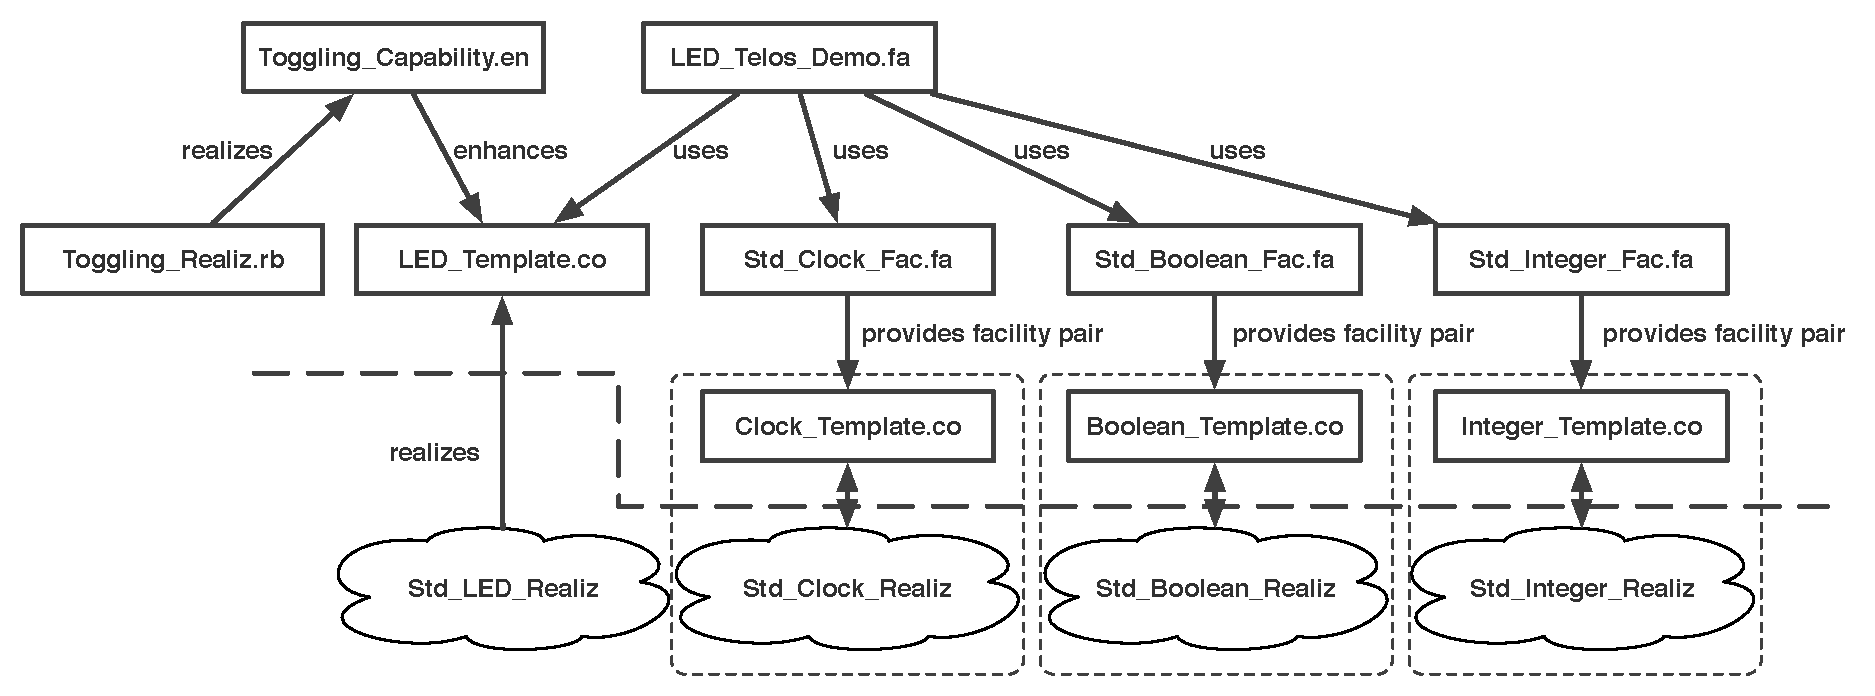
\includegraphics[scale=.55]{figs/component_graph.pdf}
\caption{A diagram illustrating inter-component relationships for the example in Section \ref{sec:specifying}}
\end{figure*}
\label{fig:imp}


Readers might note that we never presented a realization of \texttt{LED\_Template}. Indeed, after having written the concept, the RESOLVE programmer would ideally provide it with a verifiable, native RESOLVE implementation. However, as our target platform is embedded, and our concept aims to provide control for LEDs -- a decidedly low level feature on embedded hardware -- our realization is forced to operate at similarly low levels by directly manipulating hardware pins provided by msp430's chipset. 

RESOLVE, however, in its current state is too high level of a language to perform these tasks directly -- meaning it lacks the appropriate driver and language support to do so. In an effort to address this, we introduce the notion of \textit{external realizations}, which allow users to write their own realization of a concept in a language of their choosing.

The \texttt{LED\_Telos\_Demo} facility above demonstrates these developments through its use of the ``\texttt{externally realized}" phrase. This signals to the RESOLVE compiler that the user is providing a non-native realization of the \texttt{LED\_Template}, with the expectation that it conforms to the specifications dictated in the concept. 

% Applies to base types in resolve as well

% Similar to NesC, the towers of abstraction idea... eventually, similar to nesc, we get enough abstraction  through machinery such as enhancements, etc to with pieces built on top of these externally realized components.

% gives flexibility to those wishing to write other drivers and new 

We feel this new keyword is beneficial for the following reasons:
\begin{itemize}
\item The language no longer must ``hide" the fact that some of the lower level components relied upon are not written in straight-line, native RESOLVE code. The ``externally" keyword now transparently indicates this.
\item Provides flexibility for those users looking to wrap their low-level programs/drivers with formal RESOLVE interface specifications.
\end{itemize}

In the terms of embedded systems, these developments are especially as it allows us to write custom low level of the sort required for most embedded applications (e.g. LED strip drivers) while still providing formally specified interfaces that might later form the foundation . It is our hope and intention that new (native) resolve components will be layered on top of these low level, externally realized (yet specified) drivers -- eventually reaching a level of abstract where we can concern ourselves exclusively with verified, native RESOLVE components.

%In a very real sense, gives the language the capability of specifying its foundational components flexibly, and transparently which can later have all native RESOLVE components added on top. 

%More than givingHaving the freedom to use RESOLVE's specificational capabilities 

%mention performance stuff in future work section.


\begin{figure*}
\centering
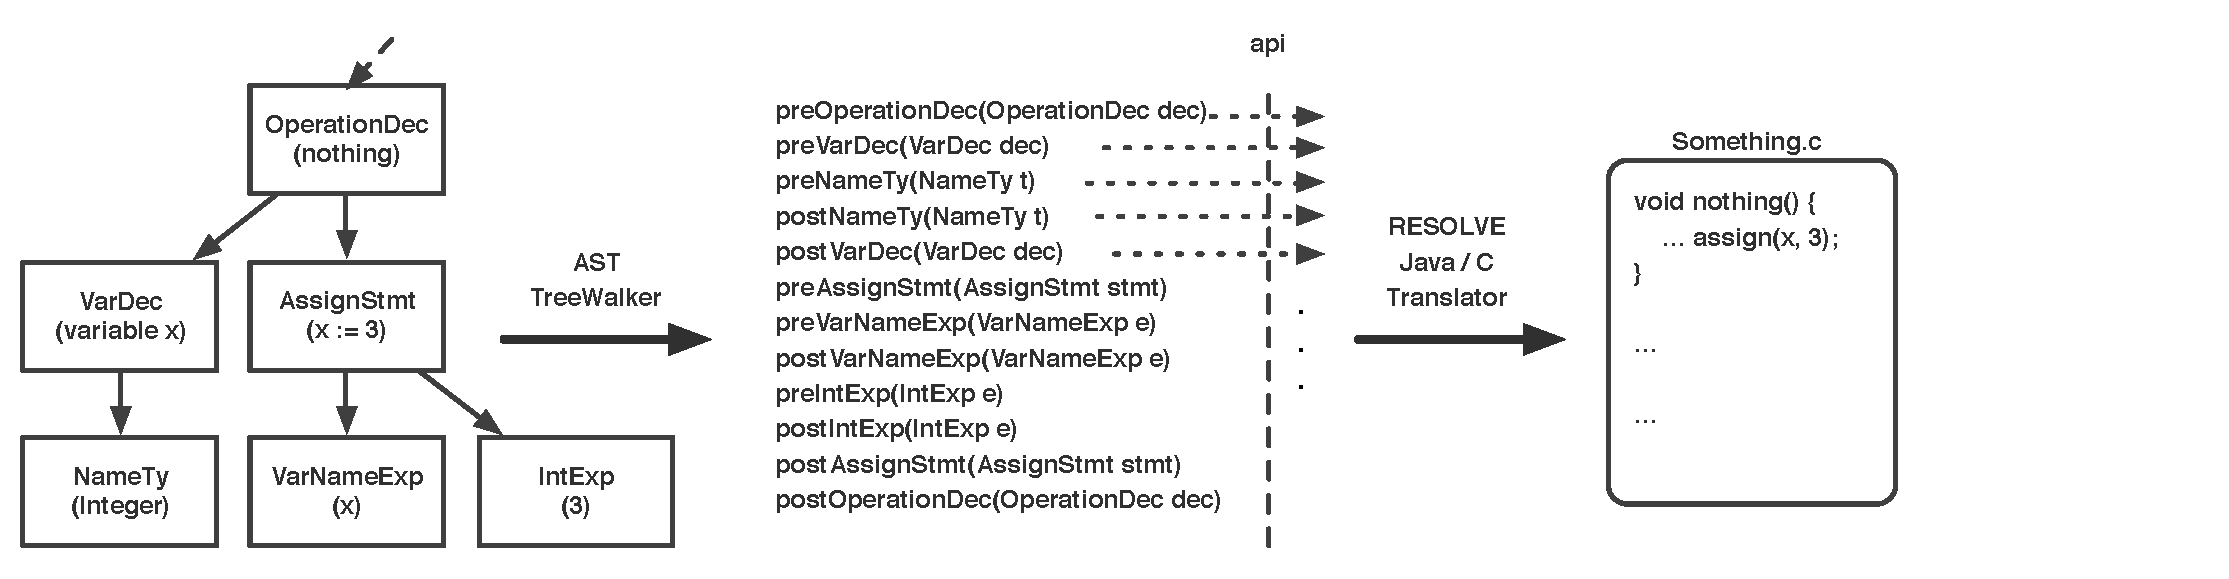
\includegraphics[scale=.55]{figs/ast_traversal.pdf}
\caption{A RESOLVE operation AST, the walk call sequence, and sample translation output.}
\end{figure*}
\label{fig:ast}

% IN THIS SECTION SHOW SOME OF OUR TRANSLATED CODE... AND WALK THROUGH IT THE SAME WAY YOU DID WITH THE CONCEPT IN RESOLVE. BUT BEFORE YOU DO THAT, SHOW THE PICTURE (The one thats already here showing high level relationships and update it!).
\section{Implementation}
Development of our C translation tool can be logically partitioned into three distinct pieces: 
\begin{enumerate}
\item Arriving at a translation model (or, strategy) for an efficient, reliable C representation of RESOLVE.
\item Implementing reusable mechanisms for carrying out the C code generation process.
\item Creation of a memory manager capable of safely allocating and freeing dynamic memory required by the generated code.
\end{enumerate}
In this section we discuss each of these phases using the LED component developed in Section \ref{sec:specifiying}.

\subsection{C Translation Model}
One of the primary challenges in translating from RESOLVE to C is finding a suitable C analog for each RESOLVE module and the constructs allowable in each. Indeed, since we are dealing with an environment where functional correctness is a primary concern, it is important that the code generated by our tool represents as closely as possible the original RESOLVE source. In an effort to make such considerations, at the highest level, the C code generated makes special considerations for facilities, concepts, and realizations. 

The memory model must also be considered as an additional verifiable component. Currently, RESOLVE is not capable of creating a complete specification of memory\footnote{RESOLVE is an object based language and has variable sized structures. Using dynamically allocatable memory is the favored approach to allow arbitrarily sized data.}. Thus, a memory model must be realized without a specification. To provide a straight forward translation from RESOLVE to C, we provide a dynamically-based memory allocator for use on embedded systems.

The relationship between the RESOLVE module type and c code generated is depicted at a high level in Figure \#. Unsurprisingly, concepts are represented in C by a single header \texttt{.h}. Some realizations connected to concepts are \texttt{externally} realized, denoting that they are not generated from RESOLVE. Additionally concepts can be \texttt{enhanced by} adding new enhancement components to the concept. RESOLVE facilities then produce corresponding \texttt{.h/c} files that provides the application interface implementation of concepts.

%Unsurprisingly, concepts are represented in C by a single header .h listing the various methods 

\subsection{Translator Implementation}

\subsubsection{AST Traversal}
Translation is performed over the course of a traversal of RESOLVE's abstract syntax tree (AST). The traversal mechanism used is a dervivative of the visitor pattern that provides a SAX-dom style pre-post traversal over all nodes in the tree. Thus, for any given node present, a total of two visits occur: One corresponding to the node being `hit' during the pre traversal stage, and one for the post. 

To make this more concrete, consider the following dummy operation.

\begin{verbatim}
Operation Nothing(); Procedure
        Var X : Integer;
        X := 3;
end Nothing;
\end{verbatim}

Shown in Figure \ref{fig:ast} is the AST representation of operation \texttt{Nothing}. Here, language constructs are represented as labeled boxes, while the actual traversal over these constructs -- and the order in which it is performed -- is communicated on the right via the call stack. Each of these calls are received in the translator in the order in which they are visited within the tree. It is up to the client (in this case, the author of the C-translator) to decide which of these methods they wish to override and perform custom actions within. 

We feel this particular traversal pattern lends itself to task of source to source translation for the following reasons:

\begin{itemize}
\item A visit method for a construct provides a convenient encapsulation of all the logic required to translate RESOLVE construct $x$ to appropriate C construct $y$.

\item Overriden visit methods apply to every instance of a construct -- meaning RESOLVE's C translator requires few (if any) loops, as the walk itself serves as the method of iteration.

\item Finally, only the visit methods for the constructs we currently wish to process need to be overridden. This makes it easy to tweak and optimize the size of the translator's codebase, implementing only visit method for language constructs that explicitly require translation.  
\end{itemize}

\subsubsection{Translation output}
Output of translated code is done using \textit{Stringtemplate} -- a third-party tool written in Java that allows users to define parameterizable templates. Like the name suggests, a template is simply ``a document with holes" that the user choses when and how to fill. 

An example C function definition template is shown below.

\begin{verbatim}
function_def(modifier, type, name, params, 
                               vars, stmts) ::= <<
<modifier> <type> <name> (<params; sep = ", ">) {
    <vars; sep = "\n">
    <stmts; sep = "\n">
}>>
\end{verbatim}

User supplied attributes, enclosed in \texttt{<..>}, indicates the position of that attribute relative to others. It is entirely up to the user to define which attributes to fill in, and how complex they want them to be. For example, the user might choose to fill the \texttt{params} attribute with a simple string, or a separately defined \texttt{parameter} template, which in turn might use another separately defined \texttt{type} template.

\begin{verbatim}
parameter(type, name) ::= "<type> <name>"
\end{verbatim}

In the context of language translation, these templates, when stored on a stack and manipulated over the course of the aforementioned AST traversal, help simplify the task of producing complicated, structured blocks of C output. For instance, upon visiting \texttt{preOperationDec}, a \texttt{function\_def} template can be instantiated by the client and pushed onto a global translation stack with its \texttt{name}, return \texttt{type}, and \texttt{modifier} attributes filled in. As \texttt{preOperationDec}'s children are visited, the \texttt{function\_def} template currently at the top of the stack receives similarly constructed parameter, variable, and statement templates from the nodes being walked. Upon reaching \texttt{postOperationDec}, we can be assured that the function has been completely filled in with the appropriate templates -- assuming the user has implemented the children's visit methods.

Hence, the only actual work being performed within visit methods is forwarding appropriate information from tree-node it represents, to an externally defined template. This allows us to exploit (in shameless design pattern parlance) a strict model view controller (MVC) separation in the translator's codebase between the mechanism that does the AST visiting (controller), the tree nodes from which we're adding information to templates (model), and the external file containing all available C language templates (view).

%One of the primary allures of this approach to translation is that that adheres to strict MVC design principles -- meaning that all output logic is distinctly separated from translation related logic. 

%We take advantage of these pre post methods using templates and simple stack to implement 


%Going even further, we demonstrate this by showing the steps taken to translate a simple operation declaration \texttt{nothing} to C.

% for each construct to remain encapsulated within that method, and (almost) completely eliminates the need for complex loop or iteration mechanisms. 


%This particular traversal pattern lends itself well to the language translation challenge (specifically source to source) where the pre methods align naturally with beginning of a construct, and conclude with its corresponding post method.  For instance, in the case above, this allows us, upon receiving a callback for In an effort to keep logic implementing our translator distinct and separate from the output language, we used a model view controller framework for implementing 

%To illustrate this, consider once again facility \texttt{DoNothing}.

\subsection{Memory Allocation}

Dynamic memory allocation does not lend itself well with an embedded programming paradigm. With hardware constraints, embedded systems have limited capacities on RAM. The telos motes are limited to 128 bytes of RAM. Many programs, however, require dynamic memory allocation to be used, including RESOLVE, in order to make it extensible. Previous RESOVE translations to C required static memory allocation \cite{regula:2010}. In this section a stack based dynamic memory allocator is introduced.

\subsubsection{Allocation using \texttt{salloc}}

The \texttt{salloc()} is a first fit memory allocator. Rather than allocating on the heap, \texttt{salloc()} uses the stack. At compilation, the allocator provisions a fixed size of memory. It requires a small section of meta-data called a block which contains information of about the size of memory allocated, neighboring blocks, as well if the block is free or not. A sample representation of the stack shown in figure \ref{fig:stack}, is a typical example of allocated memory on the stack.

\begin{figure}[!htb]
\centering
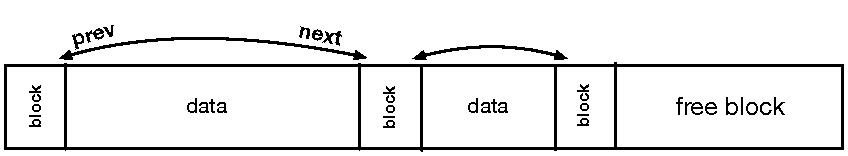
\includegraphics[scale=.55]{figs/stack.pdf}
\caption{Representation of memory stack}
\end{figure}
\label{fig:stack}

\subsubsection{Deallocation using \texttt{sfree}}

A memory allocator must provide a mechanism to release, or free memory in order to indicate that it is not being used and can be reallocated for something else. The \texttt{sfree()} operation is an analogous implementation to the standard C \texttt{free()} function for the stack.

\begin{figure}[!htb]
\centering
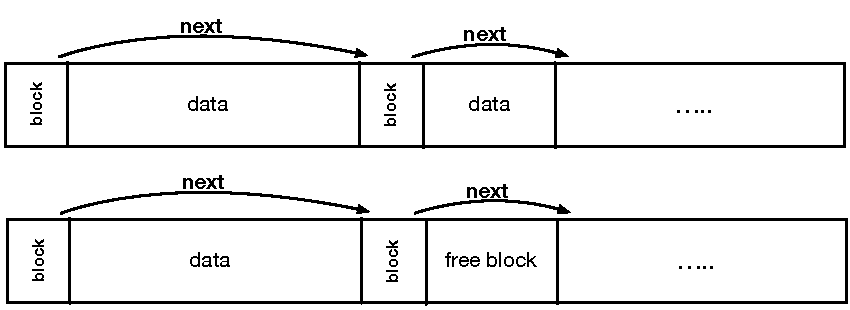
\includegraphics[scale=.55]{figs/sfree.pdf}
\caption{sfree to free memory}
\end{figure}
\label{fig:free}
 
\subsubsection{Optimizations}

A common problem that can occur in memory allocation is fragmentation.  As shown in figure \ref{fig:fragmentation}, fragmentation can lead to inefficient and increased memory usage. This problem is magnified on embedded systems with limited memory capabilities. Simple optimizations can be made however to reduce fragmentation. Splitting is one optimization that \texttt{salloc()} to maximize memory usage. Shown in figure \ref{fig:split}, blocks can be split to the size that is required. Another means of optimizing memory usage is joining together freed blocks. When a call to \texttt{sfree()} is made, neighboring blocks are coalesced together, as shown in figure \ref{fig:fuse}.

\begin{figure}[!htb]
\centering
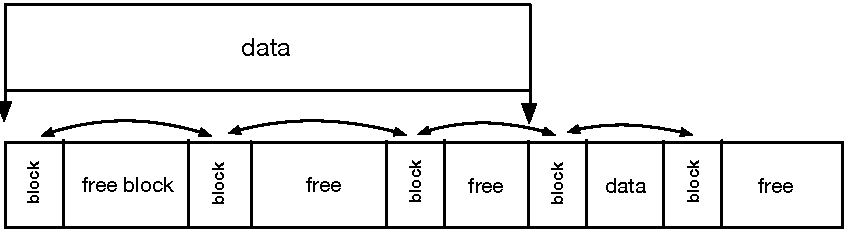
\includegraphics[scale=.55]{figs/fragmentation.pdf}
\caption{fragmentation}
\end{figure}
\label{fig:fragmentation}

\begin{figure}[!htb]
\centering
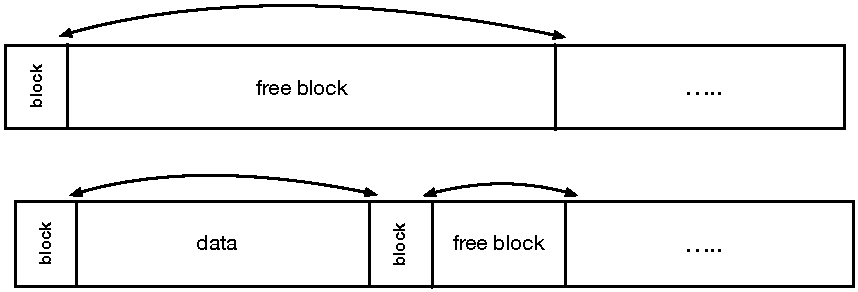
\includegraphics[scale=.55]{figs/split.pdf}
\caption{block splitting}
\end{figure}
\label{fig:split}

\begin{figure}[!htb]
\centering
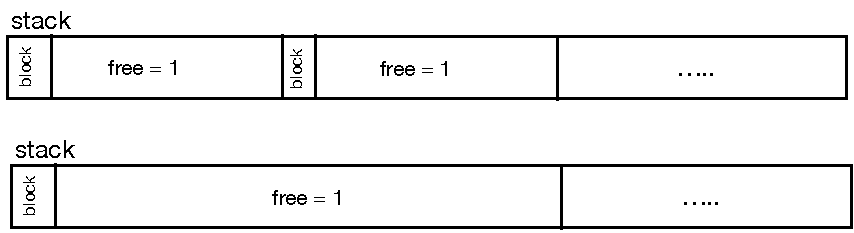
\includegraphics[scale=.55]{figs/fuse.pdf}
\caption{block fusing}
\end{figure}
\label{fig:fuse}
%A stack-based approached to dynamic memory allocation requires a fixed size of memory to be set prior to compilation. 
 
%To date there have been very few practical applications of verifiable code on physical media. 

\section{Acknowledgements}

Special thanks to Mike Kabanni, Mark Todd, and Bruce Weide whose suggestions and initial contributions in constructing the current model of RESOLVE to C translation made this work possible. 

%Open up the .tex file and compile it using Latex (Shift+Apple+L) then compile it using Bibtex (Shift+Apple+B)
\bibliographystyle{unsrt}
\bibliography{sigproc}
\end{document}